\newpage
\datos{color}{}{}
\section{[3 puntos] Ejercicio 3}
%\addcontentsline{toc}{section}{Ejercicio 1}
\textbf{Queremos modelar el siguiente problema mediante una red bayesiana. El
peso de un individuo es normal (P) si mantiene una buena alimentación (A) y realiza
ejercicio (E). Las personas que son conscientes de la importancia de la salud (S) son
más propensas a realizar ejercicio y mantener una buena alimentación. Sin embargo,
realizar ejercicio es algo que resulta más difícil si se dispone de poco tiempo libre (T).
Por último, mantener una buena alimentación reduce las posibilidades de tener alto
el colesterol (C).} \\

\textbf{Un estudio sobre los hábitos de la población revela las siguientes probabilidades:} 
\begin{multicols}{2}
\begin{itemize}
    \item \textbf{P(T) = 0,7}
    \item \textbf{P(S) = 0,4}
    \item \textbf{P(A | S) = 0,6}
    \item \textbf{P(A | ¬S) = 0,2}
    \item \textbf{P (E | S $\land$ T) = 0,5}
    \item \textbf{P (E | S $\land$ ¬T) = 0,9}
    \item \textbf{P (E | ¬S $\land$ T) = 0,2}
    \item \textbf{P (E | ¬S $\land$ ¬T) = 0,6}
\end{itemize}

\columnbreak

\begin{itemize}
    \item \textbf{P(C | A) = 0,3}
    \item \textbf{P(C | ¬A) = 0,6}
    \item \textbf{P (P | A $\land$ E) = 0,95}
    \item \textbf{P (P | A $\land$ ¬E) = 0,6}
    \item \textbf{P (P | ¬A $\land$ E) = 0,7}
    \item \textbf{P (P | ¬A $\land$ ¬E) = 0,2}
\end{itemize}
\end{multicols}


\textbf{Construye la red bayesiana que representa el problema sobre los hábitos
saludables y responde a las siguientes preguntas explicando cómo has llegado a
la solución:} \\

\begin{enumerate}[label=\alph*)]
    \item \textbf{¿Cuál es la probabilidad de tener colesterol alto (C)?}
    \item \textbf{Si una persona tiene poco tiempo libre (T) y no está concienciado sobre la
importancia de la salud (¬S), ¿qué probabilidad hay de que tenga colesterol
alto (C)?}
    \item \textbf{¿Qué probabilidad hay de que la misma persona del ejemplo anterior, sobre
la que además nos han dicho que practica ejercicio físico (E), tenga un peso
adecuado (P)?}
    \item \textbf{Responde cuál o cuáles de las siguientes afirmaciones sobre independencia
condicional son ciertas y RAZONA la respuesta dibujando el esquema de la
red. Si son dependientes, debes mostrar un camino que ilustre la dependencia entre las dos
variables sobre las que se pregunta, mientras que si son independientes, 
debes marcar los puntos que imposibilitan cada uno de los posibles caminos entre ambas.}
    \begin{enumerate}[label=\roman*.]
        \item \textbf{Si sabemos que una persona lleva una buena alimentación, pero que
dispone de poco tiempo libre, entonces conocer si está concienciado
con respecto a tener hábitos saludables, no afecta para determinar si
tendrá un buen peso.}
        \item \textbf{Si sabemos que la persona practica ejercicio, saber que dispone de
tiempo libre no nos ayuda a determinar si tiene el colesterol adecuado.}
        \item \textbf{Si sabemos que una persona concienciada sobre la importancia de la
vida saludable, lleva una buena alimentación, entonces saber si tiene
el peso adecuado ayuda a determinar si tiene el colesterol alto.}
        \item \textbf{Si sabemos que una persona lleva una buena alimentación, entonces
saber si tiene el peso adecuado ayuda a determinar si tiene el colesterol alto.}
    \end{enumerate}
\end{enumerate}


Se presenta primero la resolución manual del ejercicio y después su programación
y comprobación de resultados mediante un \textit{notebook} de \textit{Python}. En la Figura 
\ref{fig:redBayesiana} se presenta la red bayesiana que representa el problema. 
\begin{figure}[htb]
    \centering
    
\includegraphics[scale=0.5]{Images/ejer3/redBayesiana.png}
    \caption{Red bayesiana del tercer problema.} \label{fig:redBayesiana}
\end{figure}

\vspace{0.6cm}

\begin{minipage}{0.45\textwidth}
    \centering
    \begin{tabular}{c|cc}
    \toprule
    $P(S)$ & $\lnot s$ & $s$ \\
    \midrule
           & 0.6       & 0.4 \\
    \bottomrule
    \end{tabular}
    \captionof{table}{Probabilidades del nodo $S$.}
\end{minipage}\hfill
\begin{minipage}{0.45\textwidth}
    \centering
    \begin{tabular}{c|cc}
    \toprule
    $P(T)$ & $\lnot t$ & $t$ \\
    \midrule
           & 0.3       & 0.7 \\
    \bottomrule
    \end{tabular}
    \captionof{table}{Probabilidades del nodo $T$.}
\end{minipage}

\vspace{0.6cm}

% Segunda fila de tablas
\begin{minipage}{0.45\textwidth}
    \centering
    \begin{tabular}{c|cc}
    \toprule
    $P(A \mid S)$ & $\lnot a$ & $a$ \\
    \midrule
    $\lnot s$ & 0.8 & 0.2 \\
    $s$       & 0.4 & 0.6 \\
    \bottomrule
    \end{tabular}
    \captionof{table}{Probabilidades del nodo $A$.}
\end{minipage}\hfill
\begin{minipage}{0.45\textwidth}
    \centering
    \begin{tabular}{cc|cc}
    \toprule
    \multicolumn{2}{c}{$P(E \mid S,T)$} & $\lnot e$ & $e$ \\
    \midrule
    $\lnot s$ & $\lnot t$ & 0.4 & 0.6 \\
    $\lnot s$ & $t$       & 0.8 & 0.2 \\
    $s$       & $\lnot t$ & 0.1 & 0.9 \\
    $s$       & $t$       & 0.5 & 0.5 \\
    \bottomrule
    \end{tabular}
    \captionof{table}{Probabilidades del nodo $E$.}
\end{minipage}

\vspace{0.6cm}

% Tercera fila de tablas
\begin{minipage}{0.45\textwidth}
    \centering
    \begin{tabular}{c|cc}
    \toprule
    $P(C \mid A)$ & $\lnot c$ & $c$ \\
    \midrule
    $\lnot a$ & 0.4 & 0.6 \\
    $a$       & 0.7 & 0.3 \\
    \bottomrule
    \end{tabular}
    \captionof{table}{Probabilidades del nodo $C$.}
\end{minipage}\hfill
\begin{minipage}{0.45\textwidth}
    \centering
    \begin{tabular}{cc|cc}
    \toprule
    \multicolumn{2}{c}{$P(P \mid A,E)$} & $\lnot p$ & $p$ \\
    \midrule
    $\lnot a$ & $\lnot e$ & 0.8  & 0.2  \\
    $\lnot a$ & $e$       & 0.3  & 0.7  \\
    $a$       & $\lnot e$ & 0.4  & 0.6  \\
    $a$       & $e$       & 0.05 & 0.95 \\
    \bottomrule
    \end{tabular}
    \captionof{table}{Probabilidades del nodo $P$.}
\end{minipage}

\newpage
\begin{enumerate}[label=\alph*)]
\item La probabilidad de tener colesterol alto, $P(c)$, es:

Primero calculamos la probabilidad marginal de $A$ a partir de $S$:
\[
P(a) = P(a \mid s)P(s) + P(a \mid \lnot s)P(\lnot s)
     = 0.6 \cdot 0.4 + 0.2 \cdot 0.6
     = 0.24 + 0.12 = 0.36.
\]

Por tanto:
\[
P(\lnot a) = 1 - P(a) = 0.64.
\]

La probabilidad de colesterol alto se obtiene sumando sobre los valores de $A$:
\[
P(c) = P(c \mid a)P(a) + P(c \mid \lnot a)P(\lnot a)
     = 0.3 \cdot 0.36 + 0.6 \cdot 0.64.
\]

\[
P(c) = 0.108 + 0.384 = 0.492.
\]

Por tanto:
\[
P(c) = 0.492,\qquad P(\lnot c) = 0.508.
\]

La probabilidad de tener colesterol alto es aproximadamente del $49.2\%$. \\

\item Probabilidad de colesterol alto sabiendo que $t$ y $\lnot s$: $P(c \mid t \land \lnot s)$.

En la red, $C$ solo depende de $A$, y $A$ solo depende de $S$. Por tanto, dado $S$,
el nodo $T$ no influye en $C$. Podemos escribir:
\[
P(c \mid t, \lnot s) = \sum_{a \in \{a,\lnot a\}} P(c \mid a)\,P(a \mid t,\lnot s).
\]

Pero $A$ es independiente de $T$ dado $S$, así que:
\[
P(a \mid t,\lnot s) = P(a \mid \lnot s) = 0.2,\qquad
P(\lnot a \mid t,\lnot s) = P(\lnot a \mid \lnot s) = 0.8.
\]

Entonces:
\[
P(c \mid t,\lnot s) = P(c \mid a)P(a \mid \lnot s) + P(c \mid \lnot a)P(\lnot a \mid \lnot s)
= 0.3 \cdot 0.2 + 0.6 \cdot 0.8.
\]

\[
P(c \mid t,\lnot s) = 0.06 + 0.48 = 0.54.
\]

La probabilidad de colesterol alto en una persona con poco tiempo libre y no concienciada
sobre la salud es del $54\%$. \\

\item Probabilidad de peso adecuado sabiendo $t$, $\lnot s$ y $e$: $P(p \mid t,\lnot s,e)$.

El nodo $P$ depende de $A$ y $E$. Dado que conocemos $E=e$, la incertidumbre sobre $P$
proviene de $A$. Debemos calcular:
\[
P(p \mid t,\lnot s,e) = \sum_{a \in \{a,\lnot a\}} P(p \mid a,e)\,P(a \mid t,\lnot s,e).
\]

Por la estructura de la red, $A$ depende solo de $S$, y $E$ depende de $S$ y $T$.
Dado $S$ y $T$, $A$ y $E$ son independientes. Aquí conocemos $S=\lnot s$ y $T=t$,
por lo que:
\[
P(a \mid t,\lnot s,e) = P(a \mid \lnot s) = 0.2,\qquad
P(\lnot a \mid t,\lnot s,e) = P(\lnot a \mid \lnot s) = 0.8.
\]

Usando la tabla de $P$:
\[
P(p \mid a,e) = 0.95,\qquad P(p \mid \lnot a,e) = 0.7.
\]

Por tanto:
\[
P(p \mid t,\lnot s,e) = 0.95 \cdot 0.2 + 0.7 \cdot 0.8
= 0.19 + 0.56 = 0.75.
\]

La probabilidad de que esta persona tenga un peso adecuado es del $75\%$. \\

\item Afirmaciones sobre independencia condicional. Se utiliza el algoritmo de la pelota de
Bayes para determinar la independencia condicional.

\begin{enumerate}[label=\roman*.]
    \item Dado que una persona lleva buena alimentación ($a$) y tiene poco tiempo libre ($t$),
    saber si está concienciada ($s$) no afecta a la probabilidad de tener buen peso ($p$):
\[
    ¿S \perp P \mid A,T? \quad \text{o, equivalentemente,} \quad ¿P(p \mid a,t,s) = P(p \mid a,t)?
    \]

    Consideramos los caminos entre $S$ y $P$, Figura \ref{fig:d_1}:
    \begin{itemize}
        \item Camino $S \to A \to P$: $A$ es un nodo intermedio no colisionador. Como 
        es conocido, es decir, se sombrea, el camino queda bloqueado y cerrado. Por tanto, 
        las pelotas lanzadas desde $S$ no llegan a $P$. 
        \item Camino $S \to E \to P$: $E$ es un nodo intermedio no colisionador. Como 
        es desconocido, es decir, no se sombrea, el camino queda abierto y las pelotas lanzadas
        desde $S$ llegan a $P$. 
    \end{itemize}

    Existe al menos un camino abierto entre $S$ y $P$ dado $A$ y $T$, por lo que
    $S$ y $P$ son condicionalmente dependientes dado $A$ y $T$. \\

    \textbf{Conclusión:} la afirmación es \textbf{falsa}. \\

        \begin{figure}[htb]
        \centering
        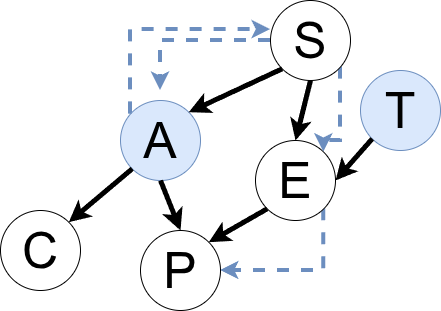
\includegraphics[scale=0.5]{Images/ejer3/d_1.png}
        \caption{Algoritmo de la pelota de Bayes para el primer supuesto.} \label{fig:d_1}
    \end{figure}

\newpage

    \item Sabiendo que la persona practica ejercicio ($e$), saber si dispone de
tiempo libre ($t$) no ayuda a determinar si tiene el colesterol adecuado ($c$):
\[
    ¿C \perp T \mid E? \quad \text{o, equivalentemente,} \quad ¿P(c \mid e,t) = P(c \mid e)?
\]

Consideramos los caminos entre $T$ y $C$, Figura \ref{fig:d_2}:
\begin{itemize}
    \item Camino $T \to E \leftarrow S \to A \to C$: en este camino, $E$ es un nodo
    colisionador (dos flechas entran en él). Si $E$ fuera desconocido, el camino
    quedaría bloqueado. Sin embargo, como $E$ es conocido ($e$), se sombrea y el
    colisionador se abre, permitiendo que las pelotas lanzadas desde $T$ lleguen
    hasta $C$ a través de $E$, $S$ y $A$.
    \item Camino $T \to E \to P \leftarrow A \to C$: en este camino, el nodo $P$ es un
    colisionador (dos flechas entran en $P$ desde $E$ y $A$). Como ni $P$ ni sus
    descendientes están condicionados, el camino queda bloqueado en $P$ y las pelotas
    lanzadas desde $T$ no pueden llegar hasta $C$ por esta ruta. 
    Además, $E$ es un nodo no colisionador condicionado, lo que también contribuye a
    bloquear el camino. Por tanto, las pelotas lanzadas desde $T$ no llegan hasta $C$ a través
    de $E$, $P$ y $A$.
\end{itemize}

Existe un camino abierto entre $T$ y $C$ dado $E$, por lo que $T$ y $C$ son
condicionalmente dependientes dado $E$. \\

\textbf{Conclusión:} la afirmación es \textbf{falsa}. \\

\begin{figure}[htb]
    \centering
    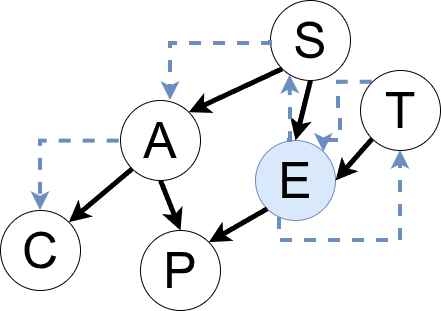
\includegraphics[scale=0.5]{Images/ejer3/d_2.png}
    \caption{Algoritmo de la pelota de Bayes para el segundo supuesto.} \label{fig:d_2}
\end{figure}

% ------------------------------------------------------------------------------

\item Sabiendo que una persona está concienciada ($s$) y lleva buena alimentación ($a$),
entonces saber si tiene el peso adecuado ($p$) ayuda a determinar si tiene colesterol alto ($c$):
\[
    ¿C \perp P \mid S,A? \quad \text{o, equivalentemente,} \quad ¿P(c \mid s,a,p) = P(c \mid s,a)?
\]

Consideramos los caminos entre $P$ y $C$, Figura \ref{fig:d_3}:
\begin{itemize}
    \item Camino $P \leftarrow A \to C$: $A$ es un nodo intermedio no colisionador y está
    en la condición (se sombrea). En el algoritmo de la pelota de Bayes, condicionar en un
    no colisionador bloquea el camino, por lo que las pelotas no pueden pasar de $P$ a $C$.
    \item Camino $P \leftarrow E \leftarrow S \to A \to C$: tanto $S$ como $A$ son nodos
    no colisionadores en este camino y ambos están condicionados (sombreados), lo que
    bloquea completamente el camino. 
\end{itemize}

Todos los caminos entre $P$ y $C$ quedan bloqueados al condicionar en $S$ y $A$, por lo que
$P$ y $C$ son condicionalmente independientes dado $S$ y $A$. \\

\textbf{Conclusión:} la afirmación es \textbf{falsa}. \\

\begin{figure}[htb]
    \centering
    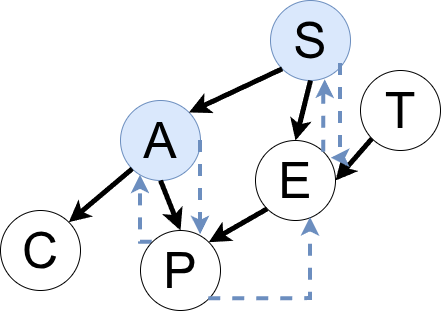
\includegraphics[scale=0.5]{Images/ejer3/d_3.png}
    \caption{Algoritmo de la pelota de Bayes para el tercer supuesto.} \label{fig:d_3}
\end{figure}

% ------------------------------------------------------------------------------

\item Sabiendo que una persona lleva buena alimentación ($a$), entonces saber si tiene
el peso adecuado ($p$) ayuda a determinar si tiene colesterol alto ($c$):
\[
    ¿C \perp P \mid A? \quad \text{o, equivalentemente,} \quad ¿P(c \mid a,p) = P(c \mid a)?
\]

Analizamos los caminos entre $P$ y $C$, Figura \ref{fig:d_4}:
\begin{itemize}
    \item Camino directo $P \leftarrow A \to C$: $A$ es un nodo no colisionador y está
    en la condición (sombreado), por lo que este camino queda bloqueado.
    \item Camino $P \leftarrow E \leftarrow S \to A \to C$: el nodo $A$ vuelve a ser un
    no colisionador en el camino y está condicionado, lo que bloquea el paso de las pelotas.
\end{itemize}

No queda ningún camino abierto entre $P$ y $C$ dado $A$, por lo que $P$ y $C$ son
condicionalmente independientes dado $A$. \\

\textbf{Conclusión:} la afirmación es \textbf{falsa}. \\

\begin{figure}[htb]
    \centering
    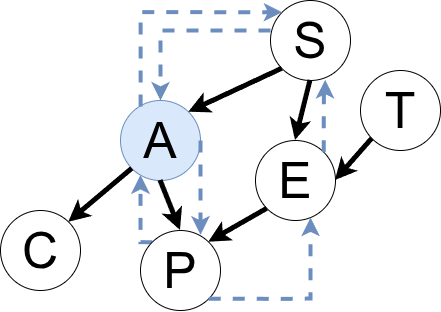
\includegraphics[scale=0.5]{Images/ejer3/d_4.png}
    \caption{Algoritmo de la pelota de Bayes para el cuarto supuesto.} \label{fig:d_4}
\end{figure}


\end{enumerate}

\end{enumerate}

\newpage
\addcontentsline{lol}{lstlisting}{3. \; \; \;\textit{Notebook} del ejercicio 3.}
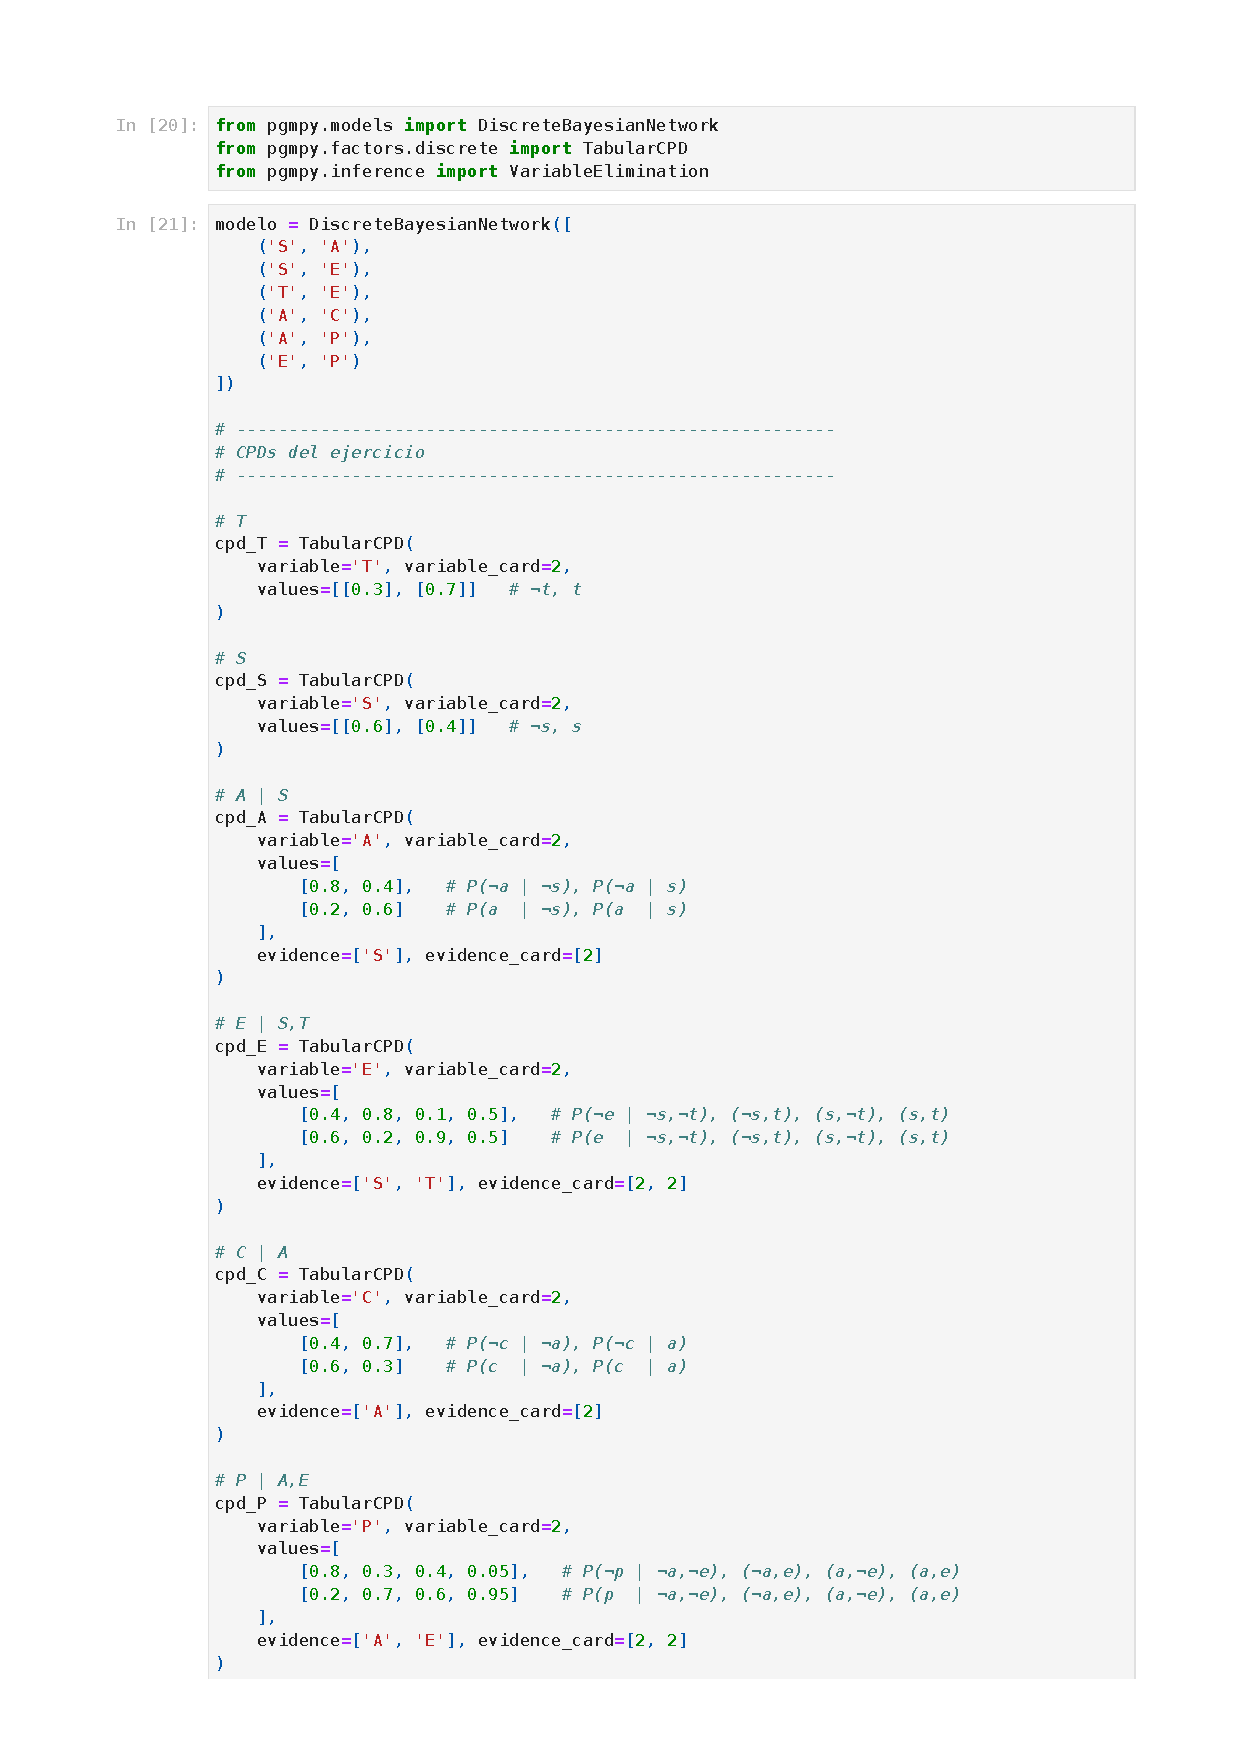
\includepdf[pages=-,pagecommand={\thispagestyle{plain}}]{Code/ejer3.pdf}